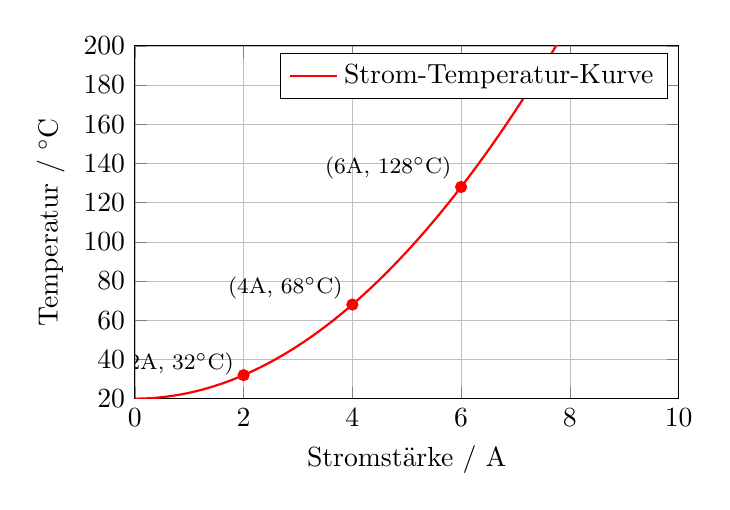
\begin{tikzpicture}
    \begin{axis}[
            xlabel={Stromstärke / A},
            ylabel={Temperatur / $^\circ$C},
            xmin=0, xmax=10,
            ymin=20, ymax=200,
            xtick={0,2,...,10},
            ytick={20,40,...,200},
            grid=both,
            major grid style={line width=.2pt,draw=gray!50},
            minor grid style={line width=.1pt,draw=gray!20},
            width=0.7\textwidth,
            height=0.5\textwidth
        ]

        % Plot für Strom-Temperatur-Kurve (nichtlinearer Zusammenhang)
        \addplot[
            color=red,
            domain=0:10,
            samples=100,
            thick,
        ] {20 + x^2 * 3};
        \addlegendentry{Strom-Temperatur-Kurve}

        % Markieren von Punkten auf der Linie
        \addplot[
            color=red,
            only marks,
            mark=*,
            mark size=2pt
        ] coordinates {
                (2,32)
                (4,68)
                (6,128)
            };

        % Beschriftungen der Punkte
        \node[anchor=south east, font=\footnotesize] at (axis cs:2,27) {($2$A, $32^\circ$C)};
        \node[anchor=south east, font=\footnotesize] at (axis cs:4,66) {($4$A, $68^\circ$C)};
        \node[anchor=south east, font=\footnotesize] at (axis cs:6,127) {($6$A, $128^\circ$C)};

    \end{axis}
\end{tikzpicture}